\documentclass[a4paper]{article}
\usepackage[english]{babel}
\usepackage[top=1.1cm,headsep=0cm,bottom=1.1cm,footskip=0cm,left=1cm,right=1cm]{geometry}
\usepackage{multicolrule} %다단 본문
\usepackage{fontspec}
\setmathtt{exprdgs-italic.ttf}[BoldFont = exprdgs-bolditalic.ttf]
\usepackage[colorlinks=true, allcolors=black]{hyperref}
\usepackage{wrapfig} %문단 내 이미지 삽입
\usepackage[abs]{overpic} %이미지 위 텍스트 삽입
\usepackage{graphicx,color} %색상
\usepackage[normalem]{ulem}%취소선
\usepackage{array} %표
\usepackage{mdframed, tcolorbox} %글상자
\usepackage{amsmath, amsfonts, amssymb, bm} %수식

\usepackage[yyyymmdd]{datetime}
\renewcommand{\dateseparator}{-}

\DeclareMathOperator{\arccsc}{arccsc}
\DeclareMathOperator{\arcsec}{arcsec}
\DeclareMathOperator{\arccot}{arccot}
\DeclareMathOperator{\csch}{csch}
\DeclareMathOperator{\sech}{sech}
\DeclareMathOperator{\arcsinh}{arcsinh}
\DeclareMathOperator{\arccosh}{arccosh}
\DeclareMathOperator{\arctanh}{arctanh}
\DeclareMathOperator{\arccsch}{arccsch}
\DeclareMathOperator{\arcsech}{arcsech}
\DeclareMathOperator{\arccoth}{arccoth}

\DeclareMathOperator{\snd}{s}
\DeclareMathOperator{\meter}{m}
\DeclareMathOperator{\cm}{cm}
\DeclareMathOperator{\mm}{mm}
\DeclareMathOperator{\mum}{\mu m}

\DeclareMathOperator{\newton}{N}
\DeclareMathOperator{\kn}{kN}
\DeclareMathOperator{\kgf}{kgf}

\DeclareMathOperator{\pa}{Pa}
\DeclareMathOperator{\kpa}{kPa}
\DeclareMathOperator{\mpa}{MPa}
\DeclareMathOperator{\gpa}{GPa}
\DeclareMathOperator{\mmhg}{mmHg}
\DeclareMathOperator{\knpm}{kN/m}

\DeclareMathOperator{\mps}{m/s}
\DeclareMathOperator{\mpss}{m/s^2}

\DeclareMathOperator{\dgr}{\!^\circ}
\DeclareMathOperator{\cel}{\!^\circ C}
\DeclareMathOperator{\fer}{\!^\circ F}
\DeclareMathOperator{\kel}{K}

\DeclareMathOperator{\kg}{kg}
\DeclareMathOperator{\kgpcm}{kg/m^3}
\DeclareMathOperator{\cmpkg}{m^3/kg}

\DeclareMathOperator{\nm}{N\cdot m}

\DeclareMathOperator{\watt}{W}
\DeclareMathOperator{\kw}{kW}
\DeclareMathOperator{\kwh}{kWh}

\DeclareMathOperator{\joule}{J}
\DeclareMathOperator{\kj}{kJ}
\DeclareMathOperator{\jpkg}{J/kg}
\DeclareMathOperator{\kjpkg}{kJ/kg}
\DeclareMathOperator{\kjpkk}{kJ/kg\cdot K}
\DeclareMathOperator{\kjpkl}{kJ/K}
\DeclareMathOperator{\kjpk}{kJ/K}
\DeclareMathOperator{\kps}{kg/s}

\DeclareMathOperator{\satat}{sat\,@}
\DeclareMathOperator{\supat}{sup\,@}
\DeclareMathOperator{\comat}{com\,@}

\usepackage{polynom} %나눗셈 필산
\usepackage{cancel} %수식 약분선
\usepackage{titlesec} %섹션 이름 변경
\usepackage{kotex} %한글
\usepackage{fancyhdr} %페이지 넘버 편집
\pagestyle{fancy}
\renewcommand{\headrulewidth}{0pt}
\fancyhf{}
\fancyhead[R]{p.\thepage}
\fancyfoot[R]{\color{red}[\LaTeX]}

\setlength\columnsep{2cm}
\SetMCRule{
	width = 0.3mm,
	color-model = rgb,
	color = {0.9,0.9,0.9},
	line-style = dashed
}

\renewcommand{\section}[1] {
	\vspace{\baselineskip}
	\noindent\hspace{-1.0cm}\begin{overpic}{qframe.png}
		\put(8mm,-0.3mm){
			\begin{tcolorbox}[
				boxsep = 0mm,
				top = 0mm,
				bottom = 0mm,
				left = 0mm,
				right = 0mm,
				boxrule = 0mm,
				colback = white,
				colframe = blue,
				width = 2.2cm,
				height = 8mm,
				halign = center,
				valign = center,
				sharp corners = all,
				opacityfill = 0,
				fontupper = \bfseries
				]
				{[ #1 ]}
			\end{tcolorbox}
		}
	\end{overpic}
}

\makeatletter
\renewcommand{\maketitle}{\setlength{\parindent}{0pt}
	\begin{flushleft}
		\LARGE{\textbf{\@title}}\\
		\vspace{0.6cm}
		\LARGE{\qquad\@author}
		\vspace{0.5cm}
	\end{flushleft}
	\hspace{-1cm}\noindent\textcolor{red}{\rule{21cm}{0.5mm}}
}
\makeatother

\newcommand{\asw}[2]{
	\begin{flushright}
		{#1 \quad #2 \quad $\blacktriangleleft$}
	\end{flushright}
}

\newcommand{\solution}{\noindent\textbf{[풀이]}}

\title{열역학(이상훈 교수님)\hspace{5cm} 2025-1 기말고사 해설}
\author{기계공학부,\quad 2022****,\quad 2학년,\quad *** \quad\begin{tabular}{ll}{\footnotesize 오류제보 : eunsoohong03@soongsil.ac.kr}\\[-11pt] {\footnotesize 작성날짜 : \today}\end{tabular}}
\date{}

\begin{document}

\maketitle

\begin{multicols*}{2}

\setlength{\parindent}{3mm}

\noindent*\;$0\cel = 273.15\kel$\\
*\;$R_{\text{Air}} = 0.287\kjpkk$\\
*\;$\kappa_{\text{Air}} = 1.4$\\
*\;$c_\mathtt{v} = 0.7175\kjpkk$\\
*\;$c_p = 1.0045\kjpkk$\\
*\;이상기체의 폴리트로픽 과정에서 :\\[5pt]
$\phantom{QU} P\mathtt{v}^n=C_1$, $T\mathtt{v}^{n-1}=C_2$, $TP^{\frac{1-n}{n}}=C_3$\\
*\;문제에서 요구한 질량보존식과 에너지 보존식을 쓸 때 문제의 조건을 적용하지 않은 기본식을 쓰시오. (하첨자 $i$, $e$ 적용 등)

\section{Q1-4}
	아래 열역학 용어들을 영어로 쓰시오.\\[10pt]
	-열효율 : thermal efficiency\\
	-C.O.P. : coefficient of performance\\
	-비가역상태 : irreversible\\
	-등엔트로피 과정 : isentropic process

\section{Q5}
	Kelvin-Plank 서술을 정의하시오.\\
	
	닫힌 과정에서 작동하는 열기관이 하나의 열원으로부터 열을 전달받아 정미일을 생산해 내는 것은 불가능하다.
	
\section{Q6}
	카르노의 원리 1번을 서술하시오.\\
	
	두 열원 사이에서 작동하는 모든 실제 열기관들의 열효율은 같은 열원 사이에서 작동하는 카르노 기관의 열효율을 넘을 수 없다.
	
\section{Q7}
	정상상태, 단일류, 개방시스템일 때 단위질량 당으로 표현한 ($a$) 열역학 제 1법칙, ($b$) 2법칙에 대한 식과 ($b$) 질량보존식을 쓰시오.
	\asw{($a$)}{$q + h_i + \frac{V_i^2}{2} + gz_i = h_e + \frac{V_e^2}{2} + gz_e + w$}
	\asw{($b$)}{$s_e = s_i + \sum \frac{q_k}{T_k} + \theta$}
	\asw{($c$)}{$\dot{m}_i = \dot{m}_e$}

\section{Q8}
	$0.6\mpa$의 포화액 상태의 수증기가 단열 팽창 밸브를 통과해서 $0.3\mpa$이 되었을 때, 밸브를 통과한 후의 수증기의 상태를 정량적으로 수치에 근거하여 결정하시오.\\
	
	\solution
	\begin{align*}
		&\cancel{q} + h_1 = h_2 + \cancel{w}\\
		&h_1 \approx h_{f@600\kpa} = 670.38\kjpkg = h_2\\
		&h_{2f} = h_{f@300\kpa} = 561.43\kjpkg
	\end{align*}
	\begin{align*}
		&h_{2g} = h_{g@300\kpa} = 2724.9\kjpkg\\
		&h_{2f} < h_2 < h_{2g}\quad\Rightarrow\quad \text{습증기}
	\end{align*}

\section{Q9}
	카르노 사이클의 정의를 서술하고 $T = T_H,\;s = s_{\text{min}}$으로 시작하는 카르노 사이클을 $T$-$s$선도에 카르노 선도를 나타내시오. (단, 열원의 온도와 각 과정에서 열전달, 모든 물리량의 단위, 4개의 상태점을 순서대로 표시하시오)\\
	
	두 개의 가역 단열과정과 두 개의 가역 등온과정으로 이루어진 사이클 상에서 작동하는 이상적인 열기관
	\begin{center}
		\includegraphics{img/fig7-19.png}
	\end{center}
	
\section{Q10}
	$80\cel$의 열원과 $25\cel$의 열원 사이에서 작동하는 카르노 열기관의 효율과 그 역과정 상에서 작동하는 카르노 열펌프의 성능 계수를 구하시오.\\
	
	\solution
	\begin{align*}
		&T_H = 80 + 273.15 = 353.15000 \approx 353.15\kel\\
		&T_H = 25 + 273.15 = 298.15000 \approx 298.15\kel\\
		&\eta_{\text{rev}} = \frac{W}{Q_H} = 1 - \frac{Q_L}{Q_H} = 1 - \frac{T_L}{T_H}\\
		&\quad = 1 - \frac{298.15}{353.15} = 0.15574119 \approx 0.156\\
		&\text{COP}_\text{R} = \frac{Q_H}{W} = \frac{1}{1 - \frac{Q_L}{Q_H}} = \frac{1}{1 - \frac{T_L}{T_H}}\\
		&\quad = \frac{1}{1-\frac{298.15}{353.15}} = 6.420909091 \approx 6.421
	\end{align*}
	\asw{}{$0.156\,;\,6.421$}

\section{Q11}
	초기 압력 $3\mpa$, 초기 온도 $270\cel$인 질량이 $5\kg$인 공기가 $n=1.25$인 폴리트로픽 과정에 의해 부피가 4.2배로 팽창한다. 이때 ($a$) 최종 온도\,[\,$\cel$], ($b$) 과정에서 공기가 한 일, ($c$) 총 엔트로피 변화를 구하시오.\\
	
	\solution
	\begin{align*}
		&T_1\mathtt{V}_1^{n-1} = T_2\mathtt{V}_2^{n-1},\quad \mathtt{V}_2 = 4.2\mathtt{V}_1\\
		&T_2 = T_1\left(\frac{\cancel{\mathtt{V}_1}}{4.2\cancel{\mathtt{V}_1}}\right)^{n-1} = 543.15\left(\frac{1}{4.2}\right)^{1.25-1}\\
		&\quad = 379.4088538 \approx 379.41\kel = 106.26\cel\\
	\end{align*}
	\asw{($a$)}{$106.26\cel$}
	\begin{align*}
		&W_{12} = m\frac{P_2\mathtt{v}_2 - P_1\mathtt{v}_1}{1-n} = \frac{mR\left(T_2 - T_1\right)}{1-n}\\
		&\quad = \frac{(5)(0.2870)(379.41-543.15)}{1 - 1.25} = 939.8676000\\
		&\quad \approx 939.868\kj
	\end{align*}
	\asw{($b$)}{$939.868\kj$}
	\begin{align*}
		&\Delta S = m\left(c_\mathtt{v}\ln\frac{T_2}{T_1} + R\ln\frac{\mathtt{V}_2}{\mathtt{V}_1}\right)\\
		&\quad = (5)\left(0.7175\ln\frac{379.41}{543.15} + (0.287)\ln(4.2)\right)\\
		&\quad = 0.772265698 \approx 0.772\kjpk
	\end{align*}
	\asw{($c$)}{$0.772\kjpk$}
	
\section{Q12}
	초기 압력 $3\mpa$, 초기 온도 $350\cel$, 초기 속도 $50\mps$인 수증기가 터빈을 통과해 최종압력은 $0.1\mpa$인 습증기가 되었다. 이때의 건도는 $92\%$이며 최종속도는 $180\mps$이다. 질량유량은 $2\kps$이며 손실열은 $15\kw$이다. ($a$) 에너지 보존식과 질량 보존식, ($b$) 축 일, ($c$) 시간 당 엔트로피의 변화량을 구하시오.\\
	
	\solution
	
	\begin{align*}
		&\dot{Q} + \dot{m}_i\left(h_i + \frac{V_i^2}{2} + gz_i\right) = \dot{m}_e\left(h_e + \frac{V_e^2}{2} + gz_i\right) + \dot{W}\\
		&\dot{m}_i = \dot{m}_e
	\end{align*}
	\begin{flushright}
		($a$)\;$\blacktriangle$
	\end{flushright}
	\begin{align*}
		&\dot{m} = \dot{m}_1 = \dot{m}_2\\
		&\dot{Q} + \dot{m}\left(h_1 + \frac{V_1^2}{2}\right) = \dot{m}\left(h_2 + \frac{V_2^2}{2}\right) + \dot{W}\\
		&T_{\satat 3\mpa} = 233.85\cel < T_1 = 350\cel\;\Rightarrow\; \text{과열증기}\\
		&h_1 = h_{@3\mpa,350\cel} = 3116.1\kjpkg\\
		&h_{2f} = h_{f\,@\,100\kpa} = 417.51\kjpkg\\
		&h_{2fg} = h_{fg\,@\,100\kpa} = 2257.5\kjpkg\\
		&h_2 = h_{2f} + x_2h_{2fg} = 417.51 + (0.92)(2257.5)\\
		&\quad = 2494.41000 \approx 2494.410\kjpkg
	\end{align*}
	\begin{align*}
		&\dot{W} = \dot{Q} + \dot{m}\left(h_1 - h_2 + \frac{V_1^2 - V_2^2}{2}\right)\\
		&\quad = -15 + (2)\left(3116.1 - 2494.41 + \frac{50^2 - 180^2}{2}\times10^{-3}\right)\\
		&\quad = 1198.48000 \approx 1198.480\kw
	\end{align*}
	\asw{($b$)}{$1198.480\kw$}
	\begin{align*}
		&s_1 = s_{@3\mpa,350\cel} = 6.7450\kjpkg\\
		&s_{2f} = s_{f\,@\,100\kpa} = 1.3028\kjpkg\\
		&s_{2fg} = s_{fg\,@\,100\kpa} = 6.0562\kjpkg\\
		&s_2 = s_{2f} + s_2h_{2fg} = 1.3028 + (0.92)(6.0562)\\
		&\quad = 6.874504000 \approx 6.875\kjpkk\\
		&\Delta S = m(s_2 - s_1) = (2)(3600)(6.875 - 6.745)\\
		&\quad = 936.000000 \approx 936.000\kjpk
	\end{align*}
	\asw{($c$)}{$936.000\kjpk$}
	
	
\section{Q13}
	정상유동의 $150\kpa$의 열 혼합기 안에서 $70\cel$의 물과 $15\cel$의 물을 혼합해 $45\cel$가 될 때, $70\cel$의 물과 $15\cel$의 물의 질량유량의 비율을 $y$라고 하자. ($y>1$) 이때 ($a$) 질량 보존식과 에너지 보존식을 구하시오. ($b$) $y$에 대한 식을 유도하고 $y$의 값을 구하시오.\\
	
	\solution
	\begin{align*}
		&\sum_i \dot{m} = \sum_e \dot{m}\\
		&\dot{Q} + \sum_i \dot{m}j = \sum_e \dot{m}j + \dot{W}
	\end{align*}
	\begin{flushright}
		($a$)\;$\blacktriangle$
	\end{flushright}
	\begin{align*}
		&\dot{m}_H = y\dot{m}_L,\quad \dot{m}_H + \dot{m}_L = \dot{m}_e\\ &\dot{m}_Hh_H + \dot{m}_Lh_L = \dot{m}_eh_e\\
		&\quad\Rightarrow\quad y\dot{m}_Lh_H + \dot{m}_Lh_L = (y\dot{m}_L + \dot{m}_L)h_e\\
		&\quad\Rightarrow\quad yh_H + h_L = (y+1)h_e\\[10pt]
		&P = 150\kpa,\quad T_1 = 70\cel,\quad T_2 = 15\cel\\
		&T_{\satat 150\kpa} = 111.35\cel > T_1 > T_e > T_2 \;\Rightarrow\;\text{압축액}\\
		&h_1 \approx h_{f\,@\,70\cel} = 293.07\kjpkg\\
		&h_2 \approx h_{f\,@\,15\cel} = 62.982\kjpkg\\
		&h_e \approx h_{f\,@\,45\cel} = 188.44\kjpkg\\
		&y = \frac{h_e - h_2}{h_1 - h_e} = \frac{188.44 - 62.982}{293.07 - 188.44} = 1.19906337 \approx 1.199
	\end{align*}
	\asw{($b$)}{$1.199$}
	
\section{Q14}
	탱크 안은 초기에 진공 상태이며 밸브가 열리고 탱크 내의 압력이 $2\mpa$에 도달하는 순간 밸브가 다시 닫힌다. 이때 ($a$) 질량보존식과 에너지 보존식을 구하시오. ($b$) $a$에서 구한 식을 이용하여 탱크 안으로 유입된 공기의 온도를 구하는 공식을 유도하시오. (단, $u\neq c_\mathtt{v}T$, $h\neq c_pT$) ($c$) 최종 온도를 구하시오.
	\begin{center}
		\includegraphics{img/q14-0.png}
	\end{center}
	\solution
	\begin{align*}
		&\sum_i m - \sum_e m = (\Delta m)_{\text{CV}}\\
		&Q + \sum_i mj - \sum_e mj - W = (\Delta E)_{\text{CV}}
	\end{align*}
	\begin{flushright}
		($a$)\;$\blacktriangle$
	\end{flushright}
	\begin{align*}
		&m_i - \cancel{m_e} = m_2 - \cancel{m_1}\\
		&\cancel{Q} + m_ih_i - \cancel{m_eh_e} - \cancel{W} = m_2u_2 - \cancel{m_1u_1}\\
		&\quad\Rightarrow\quad h_i = u_2\\
		&u_i + P_i\mathtt{v}_i = u_2\\
		&u_i + RT_i = u_2\\
		&u_2 - u_i = RT_i\\
		&c_\mathtt{v}(T_2 - T_i) = RT_i\\
		&T_2 = \left(\frac{R}{c_\mathtt{v}} + 1\right)T_i\\
		&T_2 = \left(\frac{c_p - c_\mathtt{v}}{c_\mathtt{v}} + 1\right)T_i\\
		&T_2 = \left(\frac{c_p}{c_\mathtt{v}}\right)T_i\\
		&T_2 = \kappa T_i\\
		&T_2 = (1.4)(250 + 273.15) = 732.41000\\
		&\quad \approx 732.41\kel = 459.26\cel
	\end{align*}
	
	
\section{Q15}
	$2\kg$의 공기가 최초온도 $300\kel$와 최초압력 $100\kpa$에서 최종온도 $400\kel$ 최종압력 $700\kpa$으로 수축할 때 ($a$) 공기표에서 얻은 상태량의 값으로 총 엔트로피 변화를 구하시오. ($b$) 평균 비열을 이용해 총 엔트로피 변화를 구하시오.
	\begin{center}
	\begin{tabular}{|c|c|c|}
		\hline
		$T\,[\kel]$ & $c_p\,[\kjpkk]$ & $s^\text{o}\,[\kjpkk]$\\
		\hline
		300 & 1.005 & 1.70203\\
		400 & 1.013 & 1.99194\\
		\hline
	\end{tabular}
	\end{center}
	
	\solution
	\begin{align*}
		&\Delta S = m\left(s^\text{o}_2 - s^\text{o}_1 - R\ln\frac{P_2}{P_1}\right)\\
		&\quad = (2)\left(1.99194 - 1.70203 - 0.287\ln\frac{700}{100}\right)\\
		&\quad = -0.5371324256 \approx -0.537\kjpkl
	\end{align*}
	\asw{($a$)}{$-0.537\kjpkl$}
	\begin{align*}
		&c_{p,\text{avg}} = \frac{c_{p,@300\kel} + c_{p,@400\kel}}{2} = \frac{1.005 + 1.013}{2}\\
		&\qquad = 1.009000 \approx 1.009\kjpkk\\
		&\Delta S = m\left(c_{p,\text{avg}}\ln\frac{T_2}{T_1} - R\ln\frac{P_2}{P_1}\right)\\
		&\quad = (2)\left(1.009\ln\frac{400}{300} - 0.287\ln\frac{700}{100}\right)\\
		&\quad = -0.5364100034 \approx -0.536\kjpkl
	\end{align*}
	\asw{($b$)}{$-0.536\kjpkl$}

\end{multicols*}
\end{document}